%----------
%   WARNING
%----------

% This Guide contains Library recommendations based mainly on APA and IEEE styles, but you must always follow the guidelines of your TFG Tutor and the TFG regulations for your degree.

% THIS TEMPLATE IS BASED ON THE IEEE STYLE 

% TFG - Machine Learning Based Predictive Modeling of Energy Prices

%----------
% DOCUMENT SETTINGS
%----------

\documentclass[12pt]{report} % font: 12pt

% margins: 2.5 cm top and bottom; 3 cm left and right
\usepackage[
a4paper,
vmargin=2.5cm,
hmargin=3cm
]{geometry}

% Paragraph Spacing and Line Spacing: Narrow (6 pt / 1.15 spacing) or Moderate (6 pt / 1.5 spacing)
\renewcommand{\baselinestretch}{1.15}
\parskip=6pt

% Color settings for cover and code listings 
\usepackage[table]{xcolor}
\definecolor{azulUC3M}{RGB}{0,0,102}
\definecolor{gray97}{gray}{.97}
\definecolor{gray75}{gray}{.75}
\definecolor{gray45}{gray}{.45}

% PDF/A -- Important for its inclusion in e-Archive. PDF/A is the optimal format for preservation and for the generation of metadata: http://uc3m.libguides.com/ld.php?content_id=31389625.

% In the template we include the file OUTPUT.XMPDATA. You can download that file and include the metadata that will be incorporated into the PDF file when you compile the memoria.tex file. Then upload it back to your project.
\usepackage[a-1b]{pdfx}

% LINKS
\usepackage{hyperref}
\hypersetup{colorlinks=true,
	linkcolor=black, % links to parts of the document (e.g. index) in black
	urlcolor=blue} % links to resources outside the document in blue

% MATH EXPRESSIONS
\usepackage{amsmath,amssymb,amsfonts,amsthm}

% Character encoding
\usepackage{txfonts} 
\usepackage[T1]{fontenc}
\usepackage[utf8]{inputenc}

% English settings
\usepackage[english]{babel} 
\usepackage[babel, english=american]{csquotes}
\AtBeginEnvironment{quote}{\small}

% Footer settings
\usepackage{fancyhdr}
\pagestyle{fancy}
\fancyhf{}
\renewcommand{\headrulewidth}{0pt}
\rfoot{\thepage}
\fancypagestyle{plain}{\pagestyle{fancy}}

% DESIGN OF THE TITLES of the parts of the work (chapters and epigraphs or sub-chapters)
\usepackage{titlesec}
\usepackage{titletoc}
\titleformat{\chapter}[block]
{\large\bfseries\filcenter}
{\thechapter.}
{5pt}
{\MakeUppercase}
{}
\titlespacing{\chapter}{0pt}{0pt}{*3}
\titlecontents{chapter}
[0pt]                                               
{}
{\contentsmargin{0pt}\thecontentslabel.\enspace\uppercase}
{\contentsmargin{0pt}\uppercase}                        
{\titlerule*[.7pc]{.}\contentspage}                 

\titleformat{\section}
{\bfseries}
{\thesection.}
{5pt}
{}
\titlecontents{section}
[5pt]                                               
{}
{\contentsmargin{0pt}\thecontentslabel.\enspace}
{\contentsmargin{0pt}}
{\titlerule*[.7pc]{.}\contentspage}

\titleformat{\subsection}
{\normalsize\bfseries}
{\thesubsection.}
{5pt}
{}
\titlecontents{subsection}
[10pt]                                               
{}
{\contentsmargin{0pt}                          
	\thecontentslabel.\enspace}
{\contentsmargin{0pt}}                        
{\titlerule*[.7pc]{.}\contentspage}


% Tables and figures settings
\usepackage{multirow} % combine cells 
\usepackage{caption} % customize the title of tables and figures
\usepackage{floatrow} % we use this package and its \ ttabbox and \ ffigbox macros to align the table and figure names according to the defined style.
\usepackage{array} % with this package we can define in the following line a new type of column for tables: custom width and centered content
\newcolumntype{P}[1]{>{\centering\arraybackslash}p{#1}}
\DeclareCaptionFormat{upper}{#1#2\uppercase{#3}\par}
\usepackage{graphicx}
\graphicspath{{imagenes/}} % Images folder

% Table layout for engineering
\captionsetup*[table]{
	format=upper,
	name=TABLE,
	justification=centering,
	labelsep=period,
	width=.75\linewidth,
	labelfont=small,
	font=small
}

% Figures layout for engineering
\captionsetup[figure]{
	format=hang,
	name=Fig.,
	singlelinecheck=off,
	justification=centering, % added for formatting consistency
	labelsep=period,
	labelfont=small,
	font=small		
}

% FOOTNOTES
\usepackage{chngcntr} % continuous numbering of footnotes
\counterwithout{footnote}{chapter}

% CODE LISTINGS 
% support and styling for listings. More information in  https://es.wikibooks.org/wiki/Manual_de_LaTeX/Listados_de_código/Listados_con_listings
\usepackage{listings}

% Custom listing
\lstdefinestyle{estilo}{ frame=Ltb,
	framerule=0pt,
	aboveskip=0.5cm,
	framextopmargin=3pt,
	framexbottommargin=3pt,
	framexleftmargin=0.4cm,
	framesep=0pt,
	rulesep=.4pt,
	backgroundcolor=\color{gray97},
	rulesepcolor=\color{black},
	%
	basicstyle=\ttfamily\footnotesize,
	keywordstyle=\bfseries,
	stringstyle=\ttfamily,
	showstringspaces = false,
	commentstyle=\color{gray45},     
	%
	numbers=left,
	numbersep=15pt,
	numberstyle=\tiny,
	numberfirstline = false,
	breaklines=true,
	xleftmargin=\parindent
}

\captionsetup*[lstlisting]{font=small, labelsep=period}

\lstset{style=estilo}
\renewcommand{\lstlistingname}{\uppercase{Código}}


% REFERENCES 

% IEEE bibliography setup
\usepackage[backend=biber, style=ieee, isbn=false,sortcites, maxbibnames=6, minbibnames=1]{biblatex} % Setting for IEEE citation style, recommended for engineering. "maxbibnames" indicates that from 6 authors truncate the list in the first one (minbibnames) and add "et al." as used in the IEEE style.

\addbibresource{referencias.bib} % The references.bib file in which the bibliography used should be


% MY ADDITIONS
% BLOCK DIAGRAMS
% \usepackage{tikz}
% \usetikzlibrary{shapes.geometric, arrows.meta, positioning}

\usepackage{tikz}
\usetikzlibrary{positioning, shapes.geometric, arrows.meta, fit}  % Ensure 'fit' is included

\tikzstyle{process} = [rectangle, minimum width=3.5cm, minimum height=1cm, text centered, draw=black, fill=blue!10] % Maybe get rid of the blue
\tikzstyle{arrow} = [thick,->,>=Stealth]

% INDENT FIRST PARAGRAPH AFTER SECTION
\usepackage{indentfirst}

% CODE - https://www.overleaf.com/learn/latex/Code_listing
\usepackage{listings}

% GANTT DIAGRAM
\usepackage{pgfgantt}
% \usepackage[margin=1in]{geometry} % better margins?

% For top or lower notation in text like 14th
\usepackage{textcomp}

%----------
%	DOCUMENT
%----------

\begin{document}
\pagenumbering{roman} % Roman numerals are used in the numbering of the pages preceding the body of the work.



%----------
%	COVER
%----------	
\begin{titlepage}
	\begin{sffamily}
	\color{azulUC3M}
	\begin{center}
		\begin{figure}[H] % UC3M Logo
			\makebox[\textwidth][c]{\includegraphics[width=16cm]{logo_UC3M.png}}
		\end{figure}
		\vspace{2.5cm}
		\begin{Large}
			University Degree in Telematics Engineering\\			
			 2024-2025\\ % Academic year
			\vspace{2cm}		
			\textsl{Bachelor Thesis}
			\bigskip
			
		\end{Large}
		 	{\Huge ``Machine Learning-Based Predictive Modeling of Energy Prices''}\\
		 	\vspace*{0.5cm}
	 		\rule{10.5cm}{0.1mm}\\
			\vspace*{0.9cm}
			{\LARGE Rodrigo De Lama Fernández}\\ 
			\vspace*{1cm}
		\begin{Large}
			Emilio Parrado Hernández\\
			Madrid, España, May 31st 2025\\
		\end{Large}
	\end{center}
	\vfill
	\color{black}
	% IF OUR WORK IS TO BE PUBLISHED UNDER A CREATIVE COMMONS LICENSE, INCLUDE THESE LINES. IS THE RECOMMENDED OPTION.
	
\includegraphics[width=4.2cm]{creativecommons.png}\\ % Creative Commons Logo
    This work is licensed under Creative Commons \textbf{Attribution – Non Commercial – Non Derivatives}
	\end{sffamily}
\end{titlepage}

%- three spaces will mean next page

\newpage % blank page
\thispagestyle{empty}
\mbox{}



%----------
%	ABSTRACT AND KEYWORDS 
%----------
% summary es algo mas extendido - miro lo que diga la uni
\renewcommand\abstractname{\large\bfseries\filcenter\uppercase{Summary}}
\begin{abstract}
\thispagestyle{plain}
\setcounter{page}{3}
	
	% Write your abstract
    This project focuses on the development of a machine learning-based predictive model for electricity prices in Spain. Using historical data from the OMIE (\textit{Operador del Mercado Ibérico de Energía}) and technical analysis (TA) indicators, the model aims to accurately forecast hourly energy prices. The study focuses on a single hourly slot, evaluating the performance of various Machine Learning models, such as linear regression, Lasso, and Random Forest. There was a strong focus on the feature engineering, employing technical analysis indicators such as moving averages, exponential moving averages, and momentum metrics. The results display the impact of tailoring the features to improve model accuracy and offer insights into the potential of data-driven approaches for energy price forecasting.

% \vspace*{length}
% \medskip
\bigskip
	\textbf{Keywords:} % add the keywords
            
            Energy
            
            Machine Learning
            
            Sliding Window

            Technical Analysis (TA)

            % Add more keywords
            
            % NOT RELEVANT
            % o	Forecasting
            % o	Predictive Modeling
            % o	Neural networks
	
	\vfill
\end{abstract}



\newpage % Blank page
\thispagestyle{empty}
\mbox{}



%----------
%	Dedication
%----------	
\chapter*{Dedication}

\setcounter{page}{5}

% Write here
\noindent Dedicated to my late grandfather, who was not able to see me become an engineer like himself.\\
To my amazing family.\\
To my parents, that have always helped me push through hard moments.\\
To my grandparents who will proudly see me become an engineer.\\
To my amazing girlfriend that has supported me though all the ups and downs of life.\\
To my all of friends and colleagues that have accompanied me these years.\\
To anyone and everyone that has supported me during my years in university.\\

\noindent Here is to the next steps in life

	\vfill



\newpage % blank page
\thispagestyle{empty}
\mbox{}



%----------
%	TOC
%----------	

\tableofcontents
\thispagestyle{fancy}

%--- Estructura TFG (basada en tesis de mama)

    % Agradecimientos
    
    % Dedicatorias
    
    % Indice
    % -	Abstract of the research
    % -	Key words
    
    % 1.	Introduction
    % o	Why am I doing this 
    % 	Personal
    % 	Professional
    % 2.	Marco teorico
    % a.	Teoría de los modelos preditivos
    % b.	Otros estudios
    % c.	Que tipos de modelos hay (y explicar la teoría de los distintos tipos, buscando otros autores que hayan hecho estudios con dichas metodologías y citándolos)
    % i.	Technical Analysis to create a Machine Learning model (24 in parallel)
    % ii.	Time Series Forecasting
    % iii.	Neural Networks
    % 3.	MI Modelo para predecir el precio de la electricidad
    % a.	Metodologia
    % b.	Objeto de estudio
    % c.	Plan de investigación (not really pero valorar)
    % i.	objetivos
    % ii.	preguntas
    % iii.	metodologia
    % 4.	Analysis and Interpretation of the obtained results
    % 5.	Conclusiones de la investigacion y del modelo
    %   a.	Areas de investigación alternativas que se puedan investigar
    % 6.	Referencias Bibliograficas
    % 7.	Glosario de términos
    %   a.	Explicar cosas en detalle
    % 8.	Referencias

%--- Estructura de Emilio

    % Acknowledgements
    
    % Dedication (to… mom dad gf grandparents my teacher etc)
    
    % Index
    % 1.	Introduction
    %     a.	Context (del problema)
    %     b.	Motivation (de la solucion)
    %     c.	Objectives
    %     d.	Summary of the results
    % 2.	Background
    %     a.	Description of the different componentes que uso a modo sencillo - eg modelos etc
    %     b.	ML
    %     c.	Energia
    % 3.	Proposal - si me cambian los datos este capitulo no deberia cambiar
    %     a.	Theoretical system description - esto es como juntas estos componentes - la matriz, el feature selection, los modelos especificos
    %     b. si es una limpieza generica en el tres
    % 4.	Experimentation
    %     a.	Data Description - descripcion de datos y parametros de los resultados - si es una limpieza especifica en el 4
    %     b.	Set Up Explanation - para el RF que rangos de parametros voy a hacer, dias y profundidad, validacion cruzada etc
    %     c.	Results 
    %     d.	Low level discussion
    % 5.	Conclusions
    %     a.	Recap
    %     b.	Revisit Objectives
    %     c.	Future Work
    %           - mejorar el error
%----------



% BLANK PAGE
\newpage % blank page
\thispagestyle{empty}
\mbox{}



%----------
% List of figures. If they are not included, comment the following lines
%----------
\listoffigures
\thispagestyle{fancy}

%     Example of figure:
%     \begin{figure}[H]
%     	\ffigbox[\FBwidth] {
%     	\caption[Name as seen in Index]{Figure name}
%     	}
%     	{
\includegraphics[scale=0.6]{imagenes/creativecommons.png}}
%     \end{figure}

%----------
% List of tables. If they are not included, comment the following lines
%----------
\listoftables
\thispagestyle{fancy}

%     Example of table:
% \begin{table}[H]
% 	\ttabbox[\FBwidth]
% 	{\caption{Lorem ipsum}}
% 	{\begin{tabular}{|c|P{1.5cm}|c|P{1.5cm}|P{2cm}|c|P{1.5cm}|P{2cm}|}
% 		\hline
% 		\multicolumn{2}{|c|}{\textbf{I}} & \multicolumn{2}{c|}{\textbf{II}} & \multicolumn{3}{c|}{\textbf{III}} & \textbf{IV} \\
% 		\hline
% 		x & y & x & y & x & y & x & y \\
% 		\hline
% 		10.0 & 8.04 & 10.0 & 9.14 & 10.0 & 7.46 & 8.0 & 6.58 \\
% 		\hline
% 		8.0 & 6.95 & 8.0 & 8.14 & 8.0 & 6.77 & 8.0 & 5.76 \\
% 		\hline
% 		13.0 & 7.58 & 13.0 & 8.74 & 13.0 & 12.74 & 8.0 & 7.71 \\
% 		\hline
% 		9.0 & 8.81 & 9.0 & 8.77 & 9.0 & 7.11 & 8.0 & 8.84 \\
% 		\hline
% 		11.0 & 8.33 & 11.0 & 9.26 & 11.0 & 7.81 & 8.0 & 8.47 \\
% 		\hline
% 		14.0 & 9.96 & 14.0 & 8.10 & 14.0 & 8.84 & 8.0 & 7.04 \\
% 		\hline
% 		6.0 & 7.24 & 6.0 & 6.13 & 6.0 & 6.08 & 8.0 & 5.25 \\
% 		\hline
% 		4.0 & 4.26 & 4.0 & 3.10 & 4.0 & 5.39 & 19.0 & 12.50 \\
% 		\hline
% 		12.0 & 10.84 & 12.0 & 9.13 & 12.0 & 8.15 & 8.0 & 5.56 \\
% 		\hline
% 		7.0 & 4.82 & 7.0 & 7.26 & 7.0 & 6.42 & 8.0 & 7.91 \\
% 		\hline
% 		5.0 & 5.68 & 5.0 & 4.74 & 5.0 & 5.73 & 8.0 & 6.89 \\
% 		\hline
% 		\multicolumn{5}{l}{Source: BOE}
% 	\end{tabular}}
% \end{table}

%----------
%	THESIS
%----------	
\clearpage
\pagenumbering{arabic} % numbering with Arabic numerals for the rest of the document.	

% IMPORTANT: Latex special characters are: # $ % & \ ^ _ { } ~. To avoid mistakes when compiling try writing \ before. For: \ use \textbackslash ; for ^ \textasciitilde and ~ \textasciicircum.

% Start writing here----------------------------------------------------



% Chapter 1 - introduction to the problem
\chapter{Introduction to the problem}
    \begin{itemize}
    \item \textbf{1. Explanation of how the price of energy works in Spain}
        \begin{itemize}
        \item a. Energy
        \item b. Prices
        \end{itemize}
    \item \textbf{2. Machine Learning - Lets run through some model overviews, which are available to choose, but without actually referencing anything}
    \end{itemize}

% We thought about different approaches such as Time-Series Forecasting, about Neural Networks but ...
Energy has increasingly become more important.
Availability is key for a modern high functioning society
In Europe we are lucky to have a really advanced and reliable network.
It is a key resource needed to succeed in the ecological transition that we are currently undergoing world wide.
Electric mobility is a key element of this process.
Electric cars, buses and trucks, need easily available and convenient sources of energy to recharge, to be able to play their role in society.
An important factor in this ever growing necessity is the price of the available energy.
But in recent times, that easy and affordable access has changed, and has become more unpredictable.
Ever since the commencement of the war between Russia and Ukraine marked and inflection point in the mostly cyclical nature of electricity prices.
Prices have gone up considerable since a couple years time, and it has been affecting everyone, from big consumers such as companies, to everyday people, having to pay a more expensive electricity bill at the end of the month.
This has become a topic of great concern, with more and more people thinking about it often.

This led me to think about pricing, how it was structured, and what to expect as an end consumer.
Could we plan our use of energy according to the price?
Could it be predicted accurately?
These were some of the questions I had that sparked my interest in looking into energy predictions.

In the initial discussions of this project, we talked about various ways to attack the problem at hand.
We thought about a variety of systems but settled on a plan to explore the predictions with the more established methods of Machine Learning.
This was done specially since it was a natural continuation of what was learned in the third year subject of Telematics Engineering, Modern Theory of Detection and Estimation.

The first idea we developed was to separate out the project in 24 blocks, one for each hour block to predict.
The reason behind splitting the data in 24 blocks was simple, we assumed that data between the same time slot across neighbor days, would be similar, or would follow a certain trend.

Focusing on the innovation side of things, we decided to simplify the problem.
Pivoting from creating an algorithm to predict hourly prices, to splitting that into the 24 blocks, and predicting a single one.
We decided on the 14\textsuperscript{th} hour of each day, since irrespective of the day of the week, or holiday, it would always be a valley period.

This kind of granular breaking up of data is similar to what a Random Forest does in order to absorb more details and create higher resolution predictions. We made this assumption based on the idea that it would simplify the project substantially.
% This forced us to generalize our approach, creating a system to analyze and evaluate the data in 24 distinct blocks, figuring out the best matrix dimensions for our linear regression matrix.

Talk about Emilio's background in investment banking at BBVA and his alorithms.

Talk about the idea of using technical analysis for feature engineering



% Chapter 2 - Background and Related Work (State of the Art???)
\chapter{Background and Related work}
% \begin{itemize}
% \item \textbf{References}
%     \begin{itemize}
%         \item How is the price of electricity / energy set? What happens if new producers enter the market?
%         \item Articles that reference energy prices prediction as an inspiration for my own work:
%         \begin{itemize}
%             \item 5-10 articles that do/talk about similar things
%             \item Energy consumption predictions
%             \item Energy prices in other European countries (Italy, Germany, UK, France)
%             \item Longer term predictions
%             \item Predicciones de produccion
%         \end{itemize}
%         \item Describir tecnologias – explicar mas en detalle como funciona y enlaces a donde pueda averiguar el contenido
%     \end{itemize}

%     \item Referenciar que metricas uso para medir mi error etc
%     \item Referencias de donde saco los datos

%     \item Referencias a que software utilizo referencias a documentacion de sklearn etc
% \end{itemize}

\section{General background}
How is the price of electricity set in Spain and Portugal?

LEER ARTICULO \cite{precio_electricidad_edem}

The OMIE, which stands for \textit{Operador del Mercado Ibérico de Energía} sets the final energy price.


What happens when new producers enter the market and sell to the energy pool?

Comment about more typical case studies focusing on energy consumption, since that is something more consistent and predictable

\section{The Sliding Window Approach}

How do I prepare my data to utilize across different models: The Feature Matrix (weight matrix)

The sliding window theory (mini-models)

\section{Which Machine Learning models will be used}
What algorithms will I use?

- Linear Regression: \url{https://scikit-learn.org/stable/modules/generated/sklearn.linear_model.LinearRegression.html}
% Ordinary least squares Linear Regression.

% LinearRegression fits a linear model with coefficients w = (w1, …, wp) to minimize the residual sum of squares between the observed targets in the dataset, and the targets predicted by the linear approximation.


- Lasso Regression: \url{https://scikit-learn.org/stable/modules/generated/sklearn.linear_model.Lasso.html}

The regularization strength alpha controls how much the model penalizes large coefficients. Larger alpha → more shrinkage (simpler model, potentially more bias).


% Linear Model trained with L1 prior as regularizer (aka the Lasso).

% The optimization objective for Lasso is:

% (1 / (2 * n_samples)) * ||y - Xw||^2_2 + alpha * ||w||_1

% Technically the Lasso model is optimizing the same objective function as the Elastic Net with l1_ratio=1.0 (no L2 penalty).


% The algorithm used to fit the model is coordinate descent.

% To avoid unnecessary memory duplication the X argument of the fit method should be directly passed as a Fortran-contiguous numpy array.

% Regularization improves the conditioning of the problem and reduces the variance of the estimates. Larger values specify stronger regularization. Alpha corresponds to 1 / (2C) in other linear models such as LogisticRegression or LinearSVC. If an array is passed, penalties are assumed to be specific to the targets. Hence they must correspond in number.

% The precise stopping criteria based on tol are the following: First, check that that maximum coordinate update, i.e. 
%  is smaller than tol times the maximum absolute coefficient, 
% . If so, then additionally check whether the dual gap is smaller than tol times
% .

% The target can be a 2-dimensional array, resulting in the optimization of the following objective:

% (1 / (2 * n_samples)) * ||Y - XW||^2_F + alpha * ||W||_11

% where 
%  is the sum of the magnitude of the matrix coefficients. It should not be confused with MultiTaskLasso which instead penalizes the 
%  norm of the coefficients, yielding row-wise sparsity in the coefficients.


- Random Forest: \url{https://scikit-learn.org/stable/modules/generated/sklearn.ensemble.RandomForestRegressor.html}
% A random forest regressor.

% A random forest is a meta estimator that fits a number of decision tree regressors on various sub-samples of the dataset and uses averaging to improve the predictive accuracy and control over-fitting. Trees in the forest use the best split strategy, i.e. equivalent to passing splitter="best" to the underlying DecisionTreeRegressor. The sub-sample size is controlled with the max_samples parameter if bootstrap=True (default), otherwise the whole dataset is used to build each tree.

% For a comparison between tree-based ensemble models see the example Comparing Random Forests and Histogram Gradient Boosting models.

% I cannot call fine tuning to feature engineering or hyperparameter tuning
% \section{Fine Tuning with Technical Analysis and Feature engineering}
\section{Model Optimization: Hyperparameter Tuning and Feature Engineering}

\textit{Hyperparameter tuning} or \textit{optimization} refers to the process of optimizing the model's training configuration parameters. These are parameters that are not learned from the data during the model training process, they are set before the training process begins and determine how the learning process of the model will develop. For \textit{Lasso/Ridge} regression, alpha is a hyperparameter that controls the strength of the regularization. For \textit{RandomForest}, \verb|n_estimators| (number of trees), \verb|max_depth| (maximum depth of each tree), \verb|min_samples_leaf| (minimum number of samples required to be at a leaf node), and \verb|max_features| are all hyperparameters. These values for any given model, and the dataset employed in its training, must be experimented in order to find the values that result in the best model performance (e.g., lowest error, highest accuracy) \cite{AWSHyperparameterTuning}.

% - Feature Engineering \& Feature Selection

% - Feature Engineering with Technical Analysis: This indicates that domain-specific features (technical indicators like moving averages, RSI, etc.) will be created from raw data.

% - Technical analysis based feature engineering

%     What is Technical Analysis?
    
%     The methodology of Technical analysis is interpreting and analyzing, movements in price using statistical data and historical patterns in order to make more accurate predictions. \cite{britannica_ta}
        
%     Technical indicators

%     Que es cada cosa y porque usarlos en vez de series temporales, porque la info temporal esta implicita en los indicadores.

%     Indicadores que capturan patrones en la serie

%     Ventaja: modelo ML mas sencillo pq las features son muy informativas vs

\textit{Feature Engineering} and \textit{Feature Selection} are crucial steps in preparing data for machine learning models. In this project a particular approach involving \textit{Feature Engineering with Technical Analysis} will be used by creating descriptive features based of raw data from raw price data. Technical Analysis, is a methodology for interpreting and analyzing price movements using statistical data and historical patterns to make more accurate predictions \cite{britannica_ta}. This involves generating technical indicators such as moving averages and indicators for momentum or volatility.

These indicators are not just arbitrary transformations, they are intended to capture the inherent patterns and temporal information implicitly embedded inside the raw price series, theoretically reducing the need for complex time series models. The intention of generating these highly informative features, is to improve the robustness of the Machine Learning models, as the indicators should encode valuable predictive signals. This allows for a more straightforward model architecture while attempting to leverage the rich temporal dynamics of the data, as proven in other fields such as financial data analysis.
    
% SMA, EMA, ROC, RSI, BBWidth \& ATR
A variety of technical indicators such as \textit{SMA}, \textit{EMA}, \textit{ROC}, \textit{RSI}, \textit{BBWidth} \& \textit{ATR} will be used. The \textit{Simple Moving Average} will be used with a variety of window sizes. A shorter SMA could be useful to identify short-term trends in energy prices, capture the recent price movements, while a longer SMA could be useful to capture long-term trends in energy prices, helping identify the overall direction of the market. The \textit{Exponential Moving Average} is similar to a simple moving average, but with the key difference being that it gives more weight to recent prices. This could be valuable to capture more immediate trends in energy prices.

\textbf{TODO:} Reference TA analysis academic book / article

    $ SMA_{3}, SMA_{5}, SMA_{7}, SMA_{14}, SMA_{30}, SMA_{90}, SMA_{180} $
    
    $ EMA_{3}, EMA_{5}, EMA_{7}, EMA_{14}, EMA_{30}  $

To measure momentum the price \textit{Rate of Change} measures the percentage change between the current price and a price from a previous time period (e.g., 1 day, 7 days ago). It helps identify momentum in the market and is useful to highlight trends or sudden shifts in energy prices. Additionally, the \textit{Relative Strength Index} is another momentum indicator. It is mainly a financial data point that can identify overbought or oversold conditions in the financial markets. Regarding its usage in the energy markets, the intention is it to track whether the price is approaching extreme values, which could indicate a reversal.

    $ ROC_{3}, ROC_{5}, ROC_{7}, ROC_{14}, ROC_{30} $
    
    $ RSI_{5}, RSI_{7}, RSI_{14}, RSI_{30} $

Finally, to measure volatility we employ indicators such as the Bollinger Band Width and the Standard Deviation.
    
    $ BBWidth_{7}, BBWidth_{14} $
    
    $ STD_{7}, STD_{14}, STD_{30}, STD_{90} $


\section{Evaluation Metrics}
How will I measure my accuracy?

Model accuracy will be measured with a variety errors:

MSE

MAE

$ R^2 $

RMSE

\section{Related Work}
Other ways of predicting energy prices instead of Machine Learning algorithms

Temporal Series?

Energy consumption predictions?


%----------------------------------



% Chapter 3 - Proposal - Theoretical System Description ?
\chapter{Proposal: Theoretical System Description}
% Theoretical System Description Proposal

This chapter will outline the design of the system developed for the project, describing the complete pipeline constructed for the system. This will be explained starting from a blank state, detailing the complete set-up process required to run the project. Following this initial configuration, the data preparation stage will be outlined. This will be continued by the feature matrix creation process, concluding with the training of the machine learning models and the chosen evaluation methods.

The following Block diagram will model in the most basic forms the system design:

% Contar los bloques empleados en cada parte – como junto las piezas para construir el sistema – mas adelante porque uso las piezas que uso

% 1 Retrieve Data from OMIE
% 2 Ingest data and create a CSV DB
% 3 Verify and Clean up the DB
% 4 Calculate Technical Indicators
% 5 Create Sliding Window Matrix for use in training that batch
% 6 Train the batch
% 7 Check out predictions of each mini-model with actual energy price for that time slot
% 8 Review error rates and compare with other iterations/ batches and other models. (part of Chapter 4)

\begin{figure}[H]
    \centering
    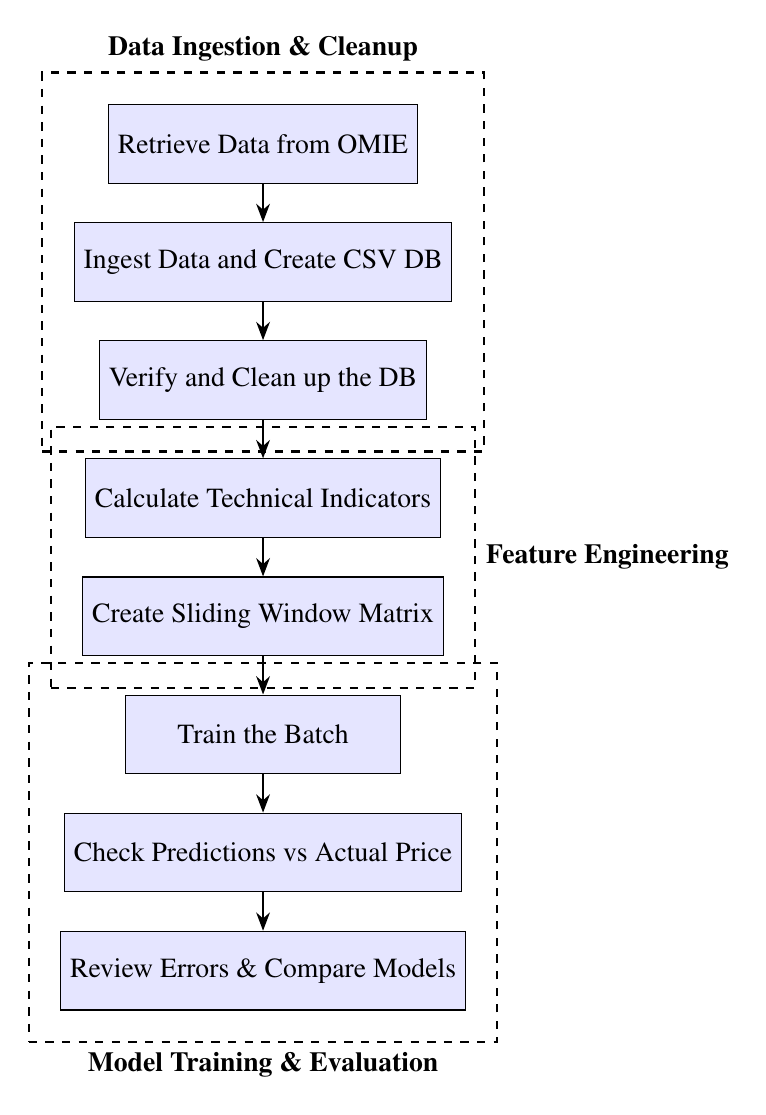
\begin{tikzpicture}[node distance=1.5cm]
    
    % Styles
    \tikzstyle{process} = [rectangle, minimum width=3.5cm, minimum height=1cm, text centered, draw=black, fill=blue!10]
    \tikzstyle{arrow} = [thick,->,>=Stealth]

    % Nodes
    \node (retrieve) [process] {Retrieve Data from OMIE};
    \node (ingest) [process, below of=retrieve] {Ingest Data and Create CSV DB};
    \node (clean) [process, below of=ingest] {Verify and Clean up the DB};
    \node (indicators) [process, below of=clean] {Calculate Technical Indicators};
    \node (matrix) [process, below of=indicators] {Create Sliding Window Matrix};
    \node (train) [process, below of=matrix] {Train the Batch};
    \node (predict) [process, below of=train] {Check Predictions vs Actual Price};
    \node (review) [process, below of=predict] {Review Errors \& Compare Models};

    % Arrows
    \draw [arrow] (retrieve) -- (ingest);
    \draw [arrow] (ingest) -- (clean);
    \draw [arrow] (clean) -- (indicators);
    \draw [arrow] (indicators) -- (matrix);
    \draw [arrow] (matrix) -- (train);
    \draw [arrow] (train) -- (predict);
    \draw [arrow] (predict) -- (review);

    % Group boxes
    \node[draw=black, thick, dashed, fit={(retrieve)(ingest)(clean)}, inner sep=0.4cm, label=above:{\textbf{Data Ingestion \& Cleanup}}] {};
        \node[draw=black, thick, dashed, fit={(indicators)(matrix)}, inner sep=0.4cm, label=right:{\textbf{Feature Engineering}}] {};
    \node[draw=black, thick, dashed, fit={(train)(predict)(review)}, inner sep=0.4cm, label=below:{\textbf{Model Training \& Evaluation}}] {};

    \end{tikzpicture}
    \caption{Theoretical Block Diagram of the Project Pipeline}
    \label{fig:block_diagram_pipeline}
\end{figure}

% Intro and preparation for the actual body of work
\section{Prior Set Up and Configuration}
% \textbf{Prior Set Up and Configuration}

Before getting into the system explanation, there are some important pre-requisites that must be met in order to run the project. The project was developed and tested with Python 3.13 \cite{python3.13}, so for any recreation of the project, it is highly recommendable to use the same version. For additional assurance of reproducibility, and as a universal best practice for Python development, it is strongly advisable to set up a new virtual environment \cite{python_venv}. Alternatively, another system that would achieve the same goal of reproducibility, and dependency conflict avoidance would be the use of Miniconda \cite{conda}. In this project we chose to use the built in Python module \textit{venv}, with which a virtual environment can be easily created and configured with the project dependencies using the following commands.

\noindent Create the virtual environment:
\begin{verbatim}
python -m venv .venv
\end{verbatim}

\noindent Activating the new virtual environment:
\begin{verbatim}
in macOS
source .venv/bin/activate

in Windows
.venv\Scripts\Activate.ps1
\end{verbatim}

\noindent To reproduce the exact environment used in the project, a \textit{requirements.txt} file must be created with the following contents:
\begin{verbatim}
ipykernel==6.29.5
matplotlib==3.10.1
numpy==2.2.3
pandas==2.2.3
requests==2.32.3
scikit-learn==1.6.1
ta==0.11.0
\end{verbatim}

\noindent To install the dependencies run:
\begin{verbatim}
pip install -r requirements.txt 
\end{verbatim}

% Should I write this in the backgorund part, or the software and licenses part?
These libraries were specifically selected to aid in the development of the project. Most of the project was written in Jupyter Notebooks, which are dependent on the \textit{ipykernel} package. To aid in the retrieval of the data, the \textit{requests} package was used to execute HTTP requests. For the manipulation of the data points, \textit{pandas} was used to house the data structures, \textit{numpy} for mathematical operations using arrays, and the \textit{ta} technical analysis library was used to compute the technical indicators. Finally the machine learning algorithms were provided by the \textit{scikit-learn} library. A special thank you is in order, dedicated to all the open source contributors of these libraries that have made this project possible

Following the completion of this prior set up required for the project, the following sections will detail in depth the different steps involved in the system pipeline.

% Three main blocks: create three sections

% Data ingestion and cleanup
\section{Data Preparation: Ingestion and Cleanup}

% General idea as a summary of what is needed in this part??

% 1. Download of OMIE data (only section independent of the whole system)
The first step in the data preparation process would be to retrieve the raw data from the original source, in this case this means downloading it from the OMIE. It is publicly available data easily discoverable through their webpage \cite{omie_datos}. The data collected was all that was initially available towards the end of 2024, with some extraordinary retrievals done later on in 2025 to complete the set with more data points.

In this scenario, it meant retrieving data from 2018 onward. While for the 5 first years available the data was self contained in a compressed archive file, the rest from 2023 to our current 2025 was not. This meant that to retrieve the files, manually downloading each resource was required. In order to streamline this process, a short Python script was created to build the necessary URIs to retrieve the files with an HTTP GET request.

The following Python script was written with modularity in mid for ease of use. It firstly creates the filenames according to the OMIE's file naming convention, inserting them into a list. This list is essential to successfully build the URIs with which the HTTP GET request will be made. Finally the function \small{\verb|download_files(urls)|} makes the request, retrieving the files.

% Insert the python script?? or better suited for an annex??
\begin{lstlisting}
import requests
from datetime import datetime, timedelta

# Usage instructions:
    # Set file name to save the filenames to download
    # Set start and end dates

file_path = 'to_download.txt'
start_date = datetime(2023, 1, 1)
end_date = datetime(2025, 3, 18)

# Compose filenames to download
def compose_filenames():
    start_date = start_date
    end_date = end_date
    
    # Generate the entries for the number of days comprehended
    to_generate = (end_date - start_date).days + 1
    entries = []
    for i in range(0, to_generate):  # x days from start to end
        date_entry = start_date + timedelta(days=i)
        entries.append(f'marginalpdbc_{date_entry.strftime("%Y%m%d")}.1')
    
    # Save to a .txt file
    with open(file_path, 'w') as file:
        for entry in entries:
            file.write(entry + '\n')

# Example URI to build
# https://www.omie.es/es/file-download?parents%5B0%5D=marginalpdbc&filename=marginalpdbc_20230102.1
def read_filenames_and_compose_urls(file_path):
    base_url = "https://www.omie.es/es/file-download?parents%5B0%5D=marginalpdbc&filename="
    
    # Read the filenames from the .txt file
    with open(file_path, 'r') as file:
        filenames = [line.strip() for line in file if line.strip()]
    
    # Compose the URLs
    urls = [base_url + filename for filename in filenames]
    
    return urls

def download_files(urls):
    for url in urls:
        # Extract the filename from the URL
        filename = url.split('=')[-1]
        
        # Send a GET request to download the file
        response = requests.get(url)
        
        # Check if the request was successful and write to file
        if response.status_code == 200:
            # Write the content to a file with the extracted filename
            with open(filename, 'wb') as file:
                file.write(response.content)
            print(f"Downloaded {filename}")
        else:
            print(f"Failed to download {filename}")

# Execution
compose_filenames()
urls = read_filenames_and_compose_urls(file_path)
download_files(urls)
\end{lstlisting}

% 2. Data Organization
The newly downloaded raw data was manually organized into its corresponding folder per year. An example filename is the following: \small{\verb|marginalpdbc_20230102.1|} This would be an important organization step for the ingestion of the data, as the next procedure involves a script that iterates through these folders, identifying all files that start with \small{\verb|marginalpdbc_|}, and parsing them into an easier to use form, a Pandas DataFrame \cite{dataframe}.

% 3. Initial Data Cleanup
When a valid file is identified while iterating through the year folders, the script reads its content. It will perform some cleanup steps, such as removing the first and last rows which are a standard header and footer across all files. It then parses the remaining data, which is separated by semicolons, into a Pandas DataFrame for that specific day. It will name the columns to \textit{Year}, \textit{Month}, \textit{Day}, \textit{Hour}, \textit{MarginalPT} (Portuguese Energy Price), and \textit{MarginalES} (Spanish Energy Price). It will also filter out any rows where the 'Year' column is not a digit, ensuring data integrity. The columns are then converted to their appropriate data types (integers for date/time components, floats for marginal prices). Each processed daily dataset is then temporarily stored in a list.

% 4. Retention of only the relevant data: Datetime and MarginalES
After processing all the individual files, the script concatenates all the daily data from the list of DataFrames into a single, comprehensive DataFrame. It will then construct a \textit{Datetime} column built from the \textit{Year}, \textit{Month}, \textit{Day}, and \textit{Hour} columns. It will also handle some peculiar cases where an \textit{Hour} value of 25 might appear (likely due to daylight savings time adjustments) by converting it to 0. This \textit{Datetime} column is then set as the DataFrame's index. Finally, it removes the individual date and hour columns as well as the \textit{MarginalPT} column, leaving only the \textit{MarginalES} as the primary target variable, along with the \textit{Datetime} index.

% 5. Final Data Cleanup and Storage
This clean and combined dataset will be saved as a CSV file for ease of use, \small{\verb|raw_data.csv|}. The script then performs further data cleanup by reloading the \small{\verb|raw_data.csv|}, and sorting it by \textit{Datetime}, saving it as \small{\verb|processed_data.csv|}. The whole process concludes by verifying the completeness of the hourly timestamps within the processed data, generating the full range of hourly timestamps that should be there, and checking for any discrepancies. If no missing timestamps are found, it confirms successful data processing; otherwise, it reports the missing timestamps, indicating an error in the data collection or processing.

For the previous in-depth explanation, you may find the following block of Python code that was created for the desired ingestion and cleanup tasks:
\begin{lstlisting}
import pandas as pd
import os

# Base path to the folder containing the year by year data folders
base_path = '../TFG/data/'

# Initialize an empty list to store DataFrames
all_data = []

# Iterate through each year folder and process all files
for root, dirs, files in os.walk(base_path):
    for file in files:
        # Check if the file starts with 'marginalpdbc_' (ignorering the rest, including the extension)
        if file.startswith('marginalpdbc_'):
            
            # Read the file
            file_path = os.path.join(root, file)
            with open(file_path, 'r', encoding='utf-8') as f:
                lines = f.readlines()

            # Remove the first line (MARGINALPDBC;) and the last line (*)
            data_lines = lines[1:-1]
            
            # Convert the list of semicolon-separated strings into a DataFrame
            daily_data = pd.DataFrame([line.strip().split(';') for line in data_lines])
            
            # Remove trailing ';' from the last column
            if daily_data.shape[1] > 6:
                # Drop empty columns
                daily_data = daily_data.iloc[:, :6]
            
            # Assign column names
            daily_data.columns = ['Year', 'Month', 'Day', 'Hour', 'MarginalPT', 'MarginalES']
            
            # Remove rows with invalid data (in case accidental empty rows or non-numeric values get included)
            daily_data = daily_data[daily_data['Year'].str.isdigit()]  # Only keep rows where 'Year' is a number
            
            # Convert the columns to the appropriate data types
            daily_data = daily_data.astype({
                'Year': int, 'Month': int, 'Day': int, 'Hour': int, 'MarginalPT': float, 'MarginalES': float
                })
            
            # Append daily data to the list
            all_data.append(daily_data)

# Concatenate all daily DataFrames into one big DataFrame
full_data = pd.concat(all_data, ignore_index=True)

# Create a datetime column from Year, Month, Day, and Hour
# Adjust the 'Hour' column to deal with the potential 25th hour issue 
full_data['Hour'] = full_data['Hour'].apply(lambda x: 0 if x == 25 else x)
full_data['Datetime'] = pd.to_datetime(full_data[['Year', 'Month', 'Day', 'Hour']], errors='coerce')

# Set the 'Datetime' column as the index
full_data.set_index('Datetime', inplace=True)

# Drop unnecessary columns
# Our target variable is 'MarginalES', so 'MarginalPT' will be dropped
full_data.drop(['Year', 'Month', 'Day', 'Hour', 'MarginalPT'], axis=1, inplace=True)

# Save the full dataset to a CSV file
full_data.to_csv('../../data/raw_data.csv')

# Database cleanup
# Load the dataset
df = pd.read_csv('../../data/raw_data.csv')

# Sort the data by the 'Datetime' column
df = df.sort_values(by='Datetime')

# Save the sorted data to a new file
df.to_csv('../../data/processed_data.csv', index=False)

# Read the CSV file
df = pd.read_csv('../../data/processed_data.csv')

# Convert 'Datetime' column to datetime objects
df['Datetime'] = pd.to_datetime(df['Datetime'])

# Generate the complete range of hourly timestamps
full_range = pd.date_range(start=df['Datetime'].min(), end=df['Datetime'].max(), freq='h')

# Find any missing timestamp
missing_timestamps = full_range.difference(df['Datetime'])

# If successful, print a message
if missing_timestamps.empty:
    print("Data processing completed successfully.")

# Else, print an error message
else:
    print("Error: Missing timestamps found. Check the data.")

    # Print missing timestamps
    print("Missing timestamps:")
    print(missing_timestamps)

    print("Data processing completed with errors.")
\end{lstlisting}

After completing this ingestion and cleanup process, the dataset will be reduced to just the 14\textsuperscript{th} hour data point. The following code will create a the final database file, which will house the singular \textit{Datetime} value, and the \textit{MarginalES} data point:

\begin{lstlisting}
import pandas as pd

# Load the original dataset
data_path = '../../data/processed_data.csv'
df = pd.read_csv(data_path, parse_dates=['Datetime'])

# Define the hour to predict and filter the data down to the 14:00H data point
hour_to_predict = 14
df_hour = df[df['Datetime'].dt.hour == hour_to_predict].copy()

# Save the final database
df_hour.to_csv("../../data/hour_14_metrics.csv", index=False)
\end{lstlisting}

To aid in the predictions, the dataset is enhanced by the used of \textit{technical analysis}, calculating a variety of technical indicators. Adding these auxiliary points of data expands the context size that our models will be able in learn from, ideally improving their prediction accuracy capabilities.

To generate these technical indicators the main database \small{\verb|processed_data.csv|} is read into a DataFrame that will be progressively expanded with new columns as new indicators are calculated. The resulting DataFrame will be saved to a secondary database \small{\verb|ta_metrics_hour_14.csv|}. The following code is an example of the process that was employed to calculate the indicators using the open source Python library \textit{ta} \cite{ta-lib}:

\begin{lstlisting}
import pandas as pd
import numpy as np
import ta  # Technical Analysis Library

# Load the data
data_path = 'data/processed_data.csv'

# Retrieve the data ensuring all data points are for the desired hour
df = pd.read_csv(data_path, parse_dates=['Datetime'])
hour_to_predict = 14
df_hour = df[df['Datetime'].dt.hour == hour_to_predict].copy()

# Simple Moving Average (SMA) (shorter window)
df_hour[f'SMA_{3}'] = ta.trend.SMAIndicator(close=df_hour['MarginalES'], window=3).sma_indicator() # last few days
df_hour[f'SMA_{5}'] = ta.trend.SMAIndicator(close=df_hour['MarginalES'], window=5).sma_indicator() # work week
df_hour[f'SMA_{7}'] = ta.trend.SMAIndicator(close=df_hour['MarginalES'], window=7).sma_indicator() # 1 week

# Simple Moving Average (longer window)
df_hour[f'SMA_{14}'] = ta.trend.SMAIndicator(close=df_hour['MarginalES'], window=14).sma_indicator() # 2 weeks
df_hour[f'SMA_{30}'] = ta.trend.SMAIndicator(close=df_hour['MarginalES'], window=30).sma_indicator() # 1 month
df_hour[f'SMA_{60}'] = ta.trend.SMAIndicator(close=df_hour['MarginalES'], window=60).sma_indicator() # 2 months
df_hour[f'SMA_{90}'] = ta.trend.SMAIndicator(close=df_hour['MarginalES'], window=90).sma_indicator() # 3 months
df_hour[f'SMA_{180}'] = ta.trend.SMAIndicator(close=df_hour['MarginalES'], window=180).sma_indicator() # 1/2 year
df_hour[f'SMA_{360}'] = ta.trend.SMAIndicator(close=df_hour['MarginalES'], window=360).sma_indicator() # 1 year

# Exponential Moving Average (EMA) (Rolling Window set as typically done in trading, attributing more weight to recent prices)
df_hour[f'EMA_{3}'] = ta.trend.EMAIndicator(close=df_hour['MarginalES'], window=3).ema_indicator()
df_hour[f'EMA_{5}'] = ta.trend.EMAIndicator(close=df_hour['MarginalES'], window=5).ema_indicator()
df_hour[f'EMA_{7}'] = ta.trend.EMAIndicator(close=df_hour['MarginalES'], window=7).ema_indicator()
df_hour[f'EMA_{14}'] = ta.trend.EMAIndicator(close=df_hour['MarginalES'], window=14).ema_indicator()
df_hour[f'EMA_{30}'] = ta.trend.EMAIndicator(close=df_hour['MarginalES'], window=30).ema_indicator()

# Rate of Change (ROC, over N days)
df_hour[f'ROC_{3}'] = ta.momentum.ROCIndicator(close=df_hour['MarginalES'], window=3).roc()
df_hour[f'ROC_{5}'] = ta.momentum.ROCIndicator(close=df_hour['MarginalES'], window=5).roc()
df_hour[f'ROC_{7}'] = ta.momentum.ROCIndicator(close=df_hour['MarginalES'], window=7).roc()
df_hour[f'ROC_{12}'] = ta.momentum.ROCIndicator(close=df_hour['MarginalES'], window=12).roc() # as done in trading for momentum
df_hour[f'ROC_{14}'] = ta.momentum.ROCIndicator(close=df_hour['MarginalES'], window=14).roc()
df_hour[f'ROC_{30}'] = ta.momentum.ROCIndicator(close=df_hour['MarginalES'], window=30).roc()

# Relative Strength Index (RSI, N-day window)
df_hour[f'RSI_{5}'] = ta.momentum.RSIIndicator(close=df_hour['MarginalES'], window=5).rsi() # rapid momentum changes
df_hour[f'RSI_{7}'] = ta.momentum.RSIIndicator(close=df_hour['MarginalES'], window=7).rsi() # rapid momentum changes
df_hour[f'RSI_{14}'] = ta.momentum.RSIIndicator(close=df_hour['MarginalES'], window=14).rsi() # standard momentum

# Drop missing values generated by rolling calculations
df_hour.dropna(inplace=True)

# Check for NaN or infinity values
print("NaN values per column:\n", df_hour.isna().sum())
print("Infinity values per column:\n", df_hour.isin([np.inf, -np.inf]).sum())

# Drop NaN or infinity values
df_hour = df_hour.replace([np.inf, -np.inf], np.nan).dropna()
# Interpolate missing values
df_hour = df_hour.interpolate()

# Check for NaN or infinity values
print("NaN values per column:\n", df_hour.isna().sum())
print("Infinity values per column:\n", df_hour.isin([np.inf, -np.inf]).sum())

# Save the dataset with metrics for the selected hour
df_hour.to_csv(f'data/ta_metrics/ta_metrics_hour_{hour_to_predict}.csv', index=False)

print(f"Metrics for hour {hour_to_predict} calculated and saved to 'data/ta_metrics/ta_metrics_hour_{hour_to_predict}.csv'.")
\end{lstlisting}

% The Feature Matrix for the Sliding Window Approach
\section{The Feature Matrix Creation}

% Theory behind feature matrices:
The creation of a \textit{feature matrix} is a key step in the process of training a supervised learning model. In this context, the objective is to structure historical energy price data into a form that can be used effectively to predict future prices. This transformation of the raw data is critical when dealing with time-series data using traditional machine learning models, since observations are ordered in time as they often exhibit autocorrelation and non-stationarity.

The intent of building the feature matrix consists on creating one unique matrix that can be used across any desired model. The feature matrix denoted as $\mathit{X}$, represents the input data used to train the model, while the target vector $\mathit{y}$ contains the values the model is intended to predict.

A simple example using only price values can be represented as:
\begin{equation*}
{X} = \begin{Bmatrix}
x_1 & x_2 & x_3 \\
x_2 & x_3 & x_4 \\
x_3 & x_4 & x_5
\end{Bmatrix}, \quad
{y} = \begin{Bmatrix}
y_1 \\
y_2 \\
y_3
\end{Bmatrix}
\end{equation*}

Here, each row of $\mathit{X}$ corresponds to a window of past values, and the corresponding element in $\mathit{y}$ is the value that follows that window, what would be the actual energy price for today:
\begin{align*}
y_1 &= x_4 \\
y_2 &= x_5 \\
y_3 &= x_6
\end{align*}

This setup reflects the temporal dependency in the time-series data, where future values are predicted based on a certain number of past observations. This approach allows machine learning models to "learn" these patterns implicit in the considered sliding window, enabling them to better predict the next value.

Incorporating technical analysis indicators to the feature matrix adds additional features such as moving averages or rate of change, enriching the model’s inputs. These indicators are calculated over historical price windows and added as extra columns to the feature matrix:

\begin{equation*}
\mathbf{X} = \begin{Bmatrix}
x_1 & x_2 & x_3 & ta_{11} & ta_{21} & \cdots & ta_{n1}\\
x_2 & x_3 & x_4 & ta_{12} & ta_{22} & \cdots & ta_{n2}\\
x_3 & x_4 & x_5 & ta_{13} & ta_{23} & \cdots & ta_{n3}
\end{Bmatrix}
\end{equation*}

Where:
\begin{itemize}
    \item $x_i$ are raw price values from previous time steps,
    \item $ta_{ij}$ is the $j$-th technical indicator calculated at time step $i$,
    \item $n$ is the number of indicators.
\end{itemize}

The target vector will remain unchanged:
\begin{equation*}
\mathbf{y} = \begin{Bmatrix}
y_1 \\
y_2 \\
y_3
\end{Bmatrix}
\end{equation*}

% The thought process behind our sliding window approach has to do with the data and the following: The dataset is NOT stationary. The data is not independent and identically distributed.
This design is motivated by the nature of the energy market data, which is \textit{non-stationary}, as the statistical properties of electricity prices (e.g., mean, variance) change over time due to evolving supply and demand dynamics, regulatory interventions, and renewable energy contributions. Since it has inherent \textit{temporal dependencies}, as prices are typically dependent on recent values, making the assumption of independent and identically distributed (i.i.d.) samples invalid. The aim is to identify \textit{local trends}, as an approach implementing sliding windows allows the model to capture short-term patterns and trends without requiring the data to be stationary.

By using a sliding window mechanism, the models will be trained on a continuous stream of overlapping data segments. This not only increases the number of training samples, enhancing generalization, but also aligning with the real-world scenario of forecasting the next value based on a recent history of observations. The ultimate aim is to build feature matrix using the sliding window approach to provide a robust and flexible representation of temporal data, allowing traditional machine learning models to operate more effectively in a domain typically reserved for time-series-specific methods.

% Non Stationary:
    
%     - Upwards trend in price: price is moving up with time according to inflation and such
    
%     - Unexpected Global events: war resulted in gas prices going way up
    
%     - Market volatility: Periods of market instability, increased renewable generation (which can lead to more volatile prices due to intermittency), or geopolitical events can cause price swings to be larger or smaller at different times.

% Not IID Independent and identically distributed:

%     - Because of the non-stationarity (trends, seasonality, changing volatility), the probability distribution from which your price data points are drawn is not the same across all observations. For example, the distribution of prices in summer will be different from winter, and the distribution during a period of high gas prices will differ from a period of low gas prices.

The following Python Script consists on the code necessary to create the simple feature matrix, which was initially generated based off \textit{MarginalES} values, with the desired sliding window width for that training batch:
\begin{lstlisting}
import pandas as pd
import numpy as np
import os

def create_feature_matrix(data, window_size):
    """
    Creates a feature matrix where each row is a sliding window of prices,
    and a corresponding target vector containing the next price value.
    
    Parameters:
    ----------
    dataframe : pandas.DataFrame
        DataFrame only containing at 'Datetime' and 'MarginalES' columns, 
    window_size : int
        Number of historical price points to include in each window
    
    Returns:
    -------
    X : pandas.DataFrame
        DataFrame with sliding windows as rows
    y : pandas.Series
        Series with target values (next price after each window)
    """
    
    # Extract the MarginalES column (assuming it's the one we want)
    if 'MarginalES' in data.columns:
        prices = data['MarginalES'].values
    else:
        # Assume it's the second column (index 1)
        prices = data.iloc[:, 1].values
    
    # Create empty matrices
    X = np.zeros((len(prices) - window_size - 1, window_size))
    y = np.zeros(len(prices) - window_size - 1)
    
    # Fill the matrices with the sliding windows and targets
    for i in range(len(prices) - window_size - 1):
        X[i, :] = prices[i:i+window_size]  # Window of prices
        y[i] = prices[i+window_size]       # Next price after window
    
    # Convert to DataFrame/Series for easier use in training
    return pd.DataFrame(X), pd.Series(y)
\end{lstlisting}

This function was later modified and extended to incorporate the extra feature columns added for as many technical indicators as desired. These were previously calculated in order to expand the context our models will be able to train with. The following code displays the flexible and auto-adaptable code for however many metrics are inputted from the secondary enhanced database that includes the technical indicators:
\begin{lstlisting}
import pandas as pd
import numpy as np
import os

def create_feature_matrix_with_features(dataframe, window_size, debug=False):
    """
    Creates a sliding window dataset for time series forecasting where each row contains:
    1. A window of historical prices (right-aligned)
    2. Feature values from the most recent point in the window
    3. Target value (next price after the window)
    
    Parameters:
    ----------
    dataframe : pandas.DataFrame
        DataFrame containing at minimum 'Datetime' and 'MarginalES' columns, 
        plus any additional feature columns
    window_size : int
        Number of historical price points to include in each window
    debug : bool, optional
        If True, print debugging information instead of using logger
        
    Returns:
    -------
    X : pandas.DataFrame
        Features DataFrame with:
        - Historical prices labeled as 'price_t-n' through 'price_t-1'
        - All additional features from the original dataframe
    y : pandas.Series
        Target values (price at time t)
    """
    
    # Input validation
    if window_size < 1:
        raise ValueError("Window size must be at least 1")
    if len(dataframe) <= window_size:
        raise ValueError(f"DataFrame must have more rows ({len(dataframe)}) than window_size ({window_size})")
    if 'Datetime' not in dataframe.columns or 'MarginalES' not in dataframe.columns:
        raise ValueError("DataFrame must contain 'Datetime' and 'MarginalES' columns")
    
    X, y = [], []
    
    # Extract price data and features
    df_prices = dataframe[['Datetime', 'MarginalES']]
    df_features = dataframe.iloc[:, 2:]  # Exclude 'Datetime' and 'MarginalES'
    feature_names = df_features.columns.tolist()
    
    if debug:
        print(f"Feature columns identified: {feature_names}")
    
    # Create samples from the data
    for i in range(window_size, len(df_prices)):
        # Extract sliding window for prices (right-aligned)
        window = df_prices.iloc[i-window_size:i, 1:].values.flatten()
        
        # Extract corresponding feature row (from the most recent point in the window)
        feature_row = df_features.iloc[i-1].values.flatten()
        
        # Concatenate sliding window prices with feature row
        X.append(np.concatenate((window, feature_row)))
        y.append(df_prices.iloc[i, 1])  # Next price point as target
    
    # Create column names for the price window
    price_columns = [f'price_t-{window_size-i}' for i in range(window_size)]
    
    # Return DataFrame with proper column names
    X_df = pd.DataFrame(X, columns=price_columns + feature_names)
    y_series = pd.Series(y, name='price_t')
    
    if debug:
        print(f"X DataFrame shape: {X_df.shape}")
        print(f"Feature columns count: {len(feature_names)}")
        print(f"Price window columns: {price_columns}")
        print(f"Total columns: {len(X_df.columns)}")
        print(f"Sample size: {len(X_df)}")
    
    return X_df, y_series
\end{lstlisting}

For an example run we can retrieve the database and select a date range:
\begin{lstlisting}
import pandas as pd
from utils.sliding_window import create_feature_matrix

# read data
csv_hour_file = '../data/hour_14_metrics.csv'
df = pd.read_csv(csv_hour_file, parse_dates=['Datetime'])
df = df[['Datetime', 'MarginalES']]

# Date range for the training matrix
train_start_date = '2018-12-25'
train_end_date = '2019-02-01'

train_subset_df = df[(df['Datetime'] >= train_start_date) & (df['Datetime'] <= train_end_date)]

# Sliding window size
window_size = 3

# Create sliding window matrix - method from utils.sliding_window
X_train, y_train = create_feature_matrix(train_subset_df, window_size)
\end{lstlisting}

We may confirm the simple matrix is correctly built with the following results:
\begin{small}
\begin{verbatim}
print(X_train.head())
       0      1      2
0  66.58  67.20  68.12
1  67.20  68.12  64.64
2  68.12  64.64  57.39
3  64.64  57.39  63.91
4  57.39  63.91  65.22

print(y_train.head())
0    64.64
1    57.39
2    63.91
3    65.22
4    65.88
\end{verbatim}
\end{small}

Furthermore, for an example run of the matrix creation with the technical indicators we can retrieve the extended database and select a date range:
\begin{lstlisting}
import pandas as pd
from utils.sliding_window import create_feature_matrix_with_features

# read data
csv_hour_file = '../data/ta_metrics/ta_metrics_hour_14.csv'
df = pd.read_csv(csv_hour_file, parse_dates=['Datetime'])
df = df[['Datetime', 'MarginalES']]

# Select all other columns except 'Datetime'
feature_columns = df.columns[1:]  # Excluding 'Datetime'
df = df[['Datetime'] + list(feature_columns)]

# Date range for the training matrix
test_start_date = '2022-01-02'
test_end_date = '2019-02-01'

train_subset_df = df[(df['Datetime'] >= train_start_date) & (df['Datetime'] <= train_end_date)]

# Sliding window size
window_size = 30

# Create sliding window matrix - method from utils.sliding_window
X_train, y_train = create_feature_matrix_with_features(train_subset_df, window_size)
\end{lstlisting}

Here we may finally confirm the matrix including the technical indicators is also correctly built:
\begin{small}
\begin{verbatim}
print(X_train.head())
   price_t-3  price_t-2  price_t-1      SMA_3   SMA_5      SMA_7  SMA_10  \
0      66.58      67.20      68.12  67.300000  66.910  66.107143  65.815   
1      67.20      68.12      64.64  66.653333  66.636  66.312857  65.674   
2      68.12      64.64      57.39  63.383333  64.786  65.225714  65.003   
3      64.64      57.39      63.91  61.980000  64.252  64.925714  64.869   
4      57.39      63.91      65.22  62.173333  63.856  64.722857  65.071   

      SMA_30   SMA_50     SMA_60  SMA_100  SMA_200     EMA_12     EMA_26  \
0  65.195000  64.9668  65.007167  66.5456  66.4343  66.023692  65.494234   
1  65.166333  64.9810  65.018333  66.4321  66.4625  65.810817  65.430958   
2  64.948000  64.8886  64.804833  66.2630  66.4792  64.515306  64.835331   
3  64.872000  65.0276  64.668333  66.1451  66.5023  64.422182  64.766788   
4  64.954000  65.0904  64.700667  66.0906  66.5257  64.544924  64.800359   

      ROC_12     ROC_50      RSI_5      RSI_7     RSI_14  
0   7.955626   9.694042  66.740433  60.838567  54.547662  
1  12.987240   1.110590  40.660255  45.129672  48.709752  
2 -17.471959  -7.450411  20.152474  27.728005  39.278321  
3  -3.239970  12.201545  49.043704  48.544816  48.866971  
4   1.747270   5.057990  53.288547  51.799200  50.556371

print(y_train.head())
0    64.64
1    57.39
2    63.91
3    65.22
4    65.88
\end{verbatim}
\end{small}

% Training of each model with the Matrix
\section{Machine Learning Model Training}

There are many strategies that can be implemented for an effective model training, depending on if the dataset is \textit{stationary} or not. An \textit{incremental} approach can be taken when de data is  \textit{stationary}, since accumulating the data points in this case the will benefit the model's training. An \textit{adaptive} approach is in order when the dataset is of \textit{non-stationary} nature. Similar to an exponential moving average, where the newer data holds more weight, while the older data's importance is progressively minimized, the model is trained on a sliding window, where the older data points are cut off. This training method "forgets" the earliest values as they are no longer relevant in order to make the latest prediction, which is is the case in the energy prices database

Having obtained fully functional matrices for both scenarios, we can use them to train each model and predict the next target value.

The generic training example is the following:
\begin{lstlisting}
import pandas as pd
from sklearn.linear_model import LinearRegression
from sklearn.linear_model import Lasso
from sklearn.ensemble import RandomForestRegressor
from sklearn.metrics import mean_squared_error, mean_absolute_error, r2_score
from sklearn.model_selection import train_test_split
from sklearn.metrics import r2_score

from utils.sliding_window import create_weight_matrix_with_features

# Load CSV
csv_hour_file = '../data/ta_metrics/metrics_hour_14.csv'
df = pd.read_csv(csv_hour_file, parse_dates=['Datetime'])

# Select features (excluding 'Datetime')
feature_columns = df.columns[1:]
df = df[['Datetime'] + list(feature_columns)]

# Filter date range
train_start_date = '2018-12-25'
train_end_date = '2021-01-01'
train_subset_df = df[(df['Datetime'] >= train_start_date) & (df['Datetime'] <= train_end_date)]

# Create sliding window matrices
window_size = 3
X, y = create_weight_matrix_with_features(train_subset_df, window_size)

# Split into training and testing sets
# Using shuffle=False since the data is a time series and needs to preserve chronology
X_train, X_test, y_train, y_test = train_test_split(X, y, test_size=0.5, shuffle=False)

# Train X-MODEL
X-MODEL = LinearRegression()
X-MODEL.fit(X_train, y_train)

# Predict on test set
y_test_pred = X-MODEL.predict(X_test)

# Evaluate performance
mse = mean_squared_error(y_test, y_test_pred)
mae = mean_absolute_error(y_test, y_test_pred)
r2 = r2_score(y_test, y_test_pred)
print(f"Test MSE: {mse:.4f}")
print(f"Test MAE: {mae:.4f}")
print(f"Test R2: {r2:.4f}")

# Predict next value based on last test row
X_last = X_test.iloc[[-1]]
y_pred_last = model.predict(X_last)[0]
y_actual_last = y_test.iloc[-1]

# Show prediction vs actual
print(f"\nLast test window input:\n{X_test.iloc[-1]}")
print(f"\nPredicted next price: {y_pred_last:.2f}")
print(f"Actual next price:    {y_actual_last:.2f}")
print(f"Prediction error:     {abs(y_pred_last - y_actual_last):.2f}")
\end{lstlisting}

With an example result of:
\begin{verbatim}
Test MSE: 51.1649
Test MAE: 5.3819
Test R2: 0.5765

Last test window input:
price_t-3    14.070000
price_t-2    39.050000
price_t-1    52.010000
SMA_3        35.043333
SMA_5        32.396000
SMA_7        30.282857
SMA_10       36.146000
SMA_30       43.679667
SMA_50       44.005000
SMA_60       43.110500
SMA_100      40.338800
SMA_200      39.112700
EMA_12       37.707358
EMA_26       40.962204
ROC_12       -3.147114
ROC_50        4.020000
RSI_5        63.118016
RSI_7        58.834894
RSI_14       54.060421
Name: 734, dtype: float64

Predicted next price: 37.55
Actual next price:    52.36
Prediction error:     14.81
\end{verbatim}

% The tested models that could be substituted into X-MODEL are the following:

% - Linear Regression: Linear combination of every feature

% - Lasso Regression: Linear model that penalizes unused features

% - Random Forest: ---

The tested models that could be substituted into \textbf{X-MODEL} are the following:
\begin{itemize}
    \item \textbf{Linear Regression}: Linear combination of every feature.
    \item \textbf{Lasso Regression}: Linear model that penalizes unused features.
    \item \textbf{Random Forest}: An ensemble learning method that constructs multiple decision trees during training and outputs the mode of the classes (for classification) or mean prediction (for regression) of the individual trees.
\end{itemize}

Review the mini model theory, why is it reasonable to not use training set, validation and test sets?

% Hablar de implementaciones como que librerías, que scripts etc – no es muy necesario, mas importante la idea ??
%----------------------------------



% Chapter 4 - Experimentation
\chapter{Experimentation}
This chapter is dedicated to reviewing all of the relevant information pertaining the experimentation phase of the project. We will review the specifics of the data that was dealt with, and explain the decisions taken for the preparation of such data, and the training of the different machine learning models employed. We will review all of the results of the different models, and discuss in depth the different set-up variations for the models.

\section{Data Description} % Data Description – OMIE data
The data that was used for this project was exclusively publicly available information, published by the OMIE (\textit{Operador del Mercado Ibérico de Energía}), the operator of the Iberian energy market. The data that was retrieved from their website \cite{omie_datos} for this project takes the following shape:

\begin{small}
\begin{verbatim}
MARGINALPDBC;
2018;01;01;1;28.1;6.74;
2018;01;01;2;33;4.74;
2018;01;01;3;32.9;3.66;
2018;01;01;4;28.1;2.3;
2018;01;01;5;27.6;2.3;
2018;01;01;6;24.6;2.06;
2018;01;01;7;20.1;2.06;
2018;01;01;8;19.9;2.06;
2018;01;01;9;19.84;2.3;
2018;01;01;10;19.9;2.3;
2018;01;01;11;19.9;2.3;
2018;01;01;12;19.9;2.3;
2018;01;01;13;23.6;2.3;
2018;01;01;14;25.1;2.3;
2018;01;01;15;23.6;5;
2018;01;01;16;24.6;5;
2018;01;01;17;25.1;5;
2018;01;01;18;27.6;8.85;
2018;01;01;19;27.6;15.93;
2018;01;01;20;28.1;22.02;
2018;01;01;21;32.9;20;
2018;01;01;22;28.1;21.95;
2018;01;01;23;28.1;23.52;
2018;01;01;24;27.6;16.35;
*
\end{verbatim}
\end{small}

We can understand and interpret this format following the OMIE's guide: \textit{Modelo de Ficheros para la distribución pública de Información del mercado de electricidad 1.35} \cite{omie_formatos_2024}. In page number 67, chapter 6.18 we may find the following information regarding the encoding format for the information:

\begin{small} % so a bit more text can appear
\begin{verbatim}
6.18 Precios marginales del mercado diario (MARGINALPDBC)

Fichero con los precios marginales del Mercado Diario para cada una de
las horas.
Nombre del fichero: marginalpdbc_aaaammdd.v donde aaaammdd
corresponde a la fecha de sesión y v es la versión del fichero.

Descripción de los campos:
CAMPO DESCRIPCIÓN VALORES VÁLIDOS
Año Año I4 – 20XX
Mes Mes I2 – 1 a 12
Día Día I2 – 1 a 31
Hora Hora I2 – 1 a 25
MarginalPT Precio marginal zona Portuguesa F8.2 – -99999.99 a 99999.99
MarginalES Precio marginal zona Española F8.2 – -99999.99 a 99999.99
\end{verbatim}
\end{small}

From this data description we can obtain the following column names: \textit{Año, Mes, Día, Hora, MarginalPT} and \textit{MarginalES}. As a proof of concept, in this investigation we will be focusing on a single time slot, simplifying the data, from multiple data points per day, to a single one. We are exclusively interested in the value of the last column, \textit{MarginalES}, and specifically the row pertaining the 14\textsuperscript{th} hour of each day, which we will refer to as 14H.
% another option 14$^{th}$

\noindent \textbf{Data analysis:}
As previously commented: the in the
No estacionario.

No son datos IID - Independientes e identicamente distribuidos.

Hay correlacion en mis datos entre cada dia? Si deberia ser relativamente alta, estacional, pero progresiva y lenta.

For the data visualization portion, I employed various methods, bot plotting values with matplotlib, seaborn and using the Microsoft Data Wrangler Visual Studio Code extension.

Explain some more about the data distribution.

Explain the ups and downs of the data (war and relation to natural gas prices).

Explain the zero price.

\section{Model Set Up Explanation}
How do I use the previously explained system - what parameters did I modify to obtain the final results. Feature engineering, Alpha variation testing in Lasso, Tree depth and number of leafs.
Que modelos y que configs

Cross validation?? Not really done, in another way w the sliding window
cambio parametros pero no la arquitectura del modelo
- Linear Regressor

- Lasso Regressor

Experimenting with alpha using a loop or GridSearchCV to find the optimal value.

- Random Forest
%como lo usas en el sentido de tocar cosas, parametros como numero de arboles profundidad, el Alpha del lasso
tune hyperparameters like n estimators, max depth, etc.

\section{Results of the Testing}
Results as graph/ tables - This would be to compare a model across various iterations. Model best-run comparisons, etc.
% a modo tabla unica comparando todas las iteraciones de cada technologia, y luego una conjunta con la mejor de todo (Si me hace falta mas, pues al apendice)

Review error rates and compare with other iterations/ batches and other models.

Error medio en todas las predicciones

Y percentiles (expectation shortfall tambien?)

\section{Discussion} % of the results
This would be the final explanation that I would give to a colleague of mine, with full details on how I have done everything
%----------------------------------



% Chapter 5 - Regulatory Framework (Marco Regulador)
\chapter{Regulatory Framework}
Not essential for this investigative project because we do not go to market.

\section{Data Availability}
Habria que hablar de las normas, pq si alguien lo usa es para ir a mercado

Current Spanish and European regulations allow for the use of publicly available institutional data for use in educational investigative work.

I need to talk about laws, what data is permissible to use and how. This would be essential for a project that does indeed go to market.

For us, its not that relevant.

\section{Software \& Licenses}

For the development of this project I have used a variety of open and closed source utilies and code.

For the sake of organization, I will categorize this section into two distinct parts, required software to reproduce the project, and optional software for ease of production, plannification, organization or otherwise related.

Required:

Python - This was the programming language in wich the entirety of the project was developed \cite{python}

Scikit-learn - library for ml \cite{scikit-learn}

Pandas - data management \cite{pandas}

ta library - Technical Analysis library\cite{ta-lib}

Light use of Seaborn - data visualization \cite{seaborn}

NumPy - number manipulation \cite{numpy}

macOS / Windows - closed source platforms across where the project was developed \cite{macos} \& \cite{windows}

Optional:

Git - a distributed version control system \cite{git}

GitHub - Repository hosting platform \cite{github}

Visual Studio Code - open source text editor for my general coding needs \cite{vscode}

Visual Studio Code extensions such as Microsoft Data Wrangler, Python packages or such

Python Virtual Environment (venv) - This was created as it is best practice to create new Python virtual environments for each new project, as specially in a production environment these usually require certain specific versions that must be met in order for all components to work as intended. An alternative method of dealing with this would be using Conda, and creating with it a new Conda environment, \cite{python_venv}

Overleaf - closed source platform used to compile LaTeX code \cite{overleaf}

LaTeX - open source language used to create the final project document \cite{latex}

OpenAI ChatGPT, Google Gemini \& Anthropic Claude - closed source large language models used to aid in troubleshooting general coding issues



% Chapter 6 - Socio-economic Environment - Entorno socio-economico
\chapter{Socio-economic Environment}
\section{Socio-economic Impact}

Why is this relevant?

- Energy Prediction

- Shutdowns

- Price sensitivity

% En este TFG, se dan algunas pinceladas sobre una posible aplicación futura de las
% redes SDN de nueva generación en entornos de defensa, concretamente en entornos de
% aviónica militar.
% Por medio de la aplicación SDN desarrollada, se han podido exponer las a la vez las
% bondades y maldades de este paradigma. Citando algunas de sus mayores bazas concep-
% tuales, el uso de las SDN con su heterogeneización de los equipos de red puede conllevar
% una drástica reducción de consumo de materias primas, al poder utilizar distintos tipos de
% hardware y poder aprovecharlos de distintas maneras a lo largo de su vida útil.
% Añadiendo a este razonamiento, las SDN habilitan la posibilidad de implantar solu-
% ciones con compatibilidad hacia atrás, algo que en entornos de defensa, al menos en la
% división de AIRBUS junto con la que se ha realizado este TFG, no se encuentra general-
% mente entre los objetivos prioritarios a la hora de desarrollar nuevos sistemas para este
% ámbito.

\section{Project plan}
TODO: Gantt diagram representing time spent in each phase - Design and innovation time frames

\begin{figure}[H]
    \centering
    \begin{ganttchart}[
        x unit=1cm, % width of one month
        y unit chart=0.8cm,
        hgrid,
        vgrid,
        time slot unit=month,
        time slot format=isodate-yearmonth,
        % compress calendar, % what is this / why is it not working?
        bar height=0.6
        ]{2024-09}{2025-06}
    
        \gantttitlecalendar{year, month=shortname} \\
    
        \ganttgroup{Project Phase 1}{2024-09}{2025-01} \\
        \ganttbar{System Design}{2024-10}{2024-12} \\
        \ganttbar{Coding}{2024-12}{2025-01} \\
    
        \ganttgroup{Project Phase 2}{2025-01}{2025-06} \\
        \ganttbar{Results Gathering}{2025-01}{2025-05} \\
        \ganttbar{Redacting the Thesis}{2025-05}{2025-06}
    
    \end{ganttchart}
    \caption{Gantt Diagram of the Project Lifecycle}
    \label{fig:gantt_diagram}
\end{figure}

\section{Budget}
This section will consist of a complete price breakdown of the investigation, consisting of material costs such as the equipment utilized, and the human capital that composed the investigation team. It is notable to highlight that as previously mentioned, no paid license of any sort was obtained for the realization of this project. All of the programs, tools or code, were either \textit{Open Source} or free to use software under exclusive \textit{non-commercial use} licenses.

The most basic requirement for the physical needs of this project is a computer with an desktop operating system. Since the project was written in Python \cite{python}, it would be reasonable to consider it platform agnostic. Any computer capable of running any recent operating system, configured with a recent version of Python would be able to run this project. This includes any of the three most popular desktop operating systems, Windows, macOS and any Linux distribution.

The project was mainly tested using Python 3.13 \cite{python3.13} which does require a recent operating system such as macOS 13 or Windows 10. But as for the project itself, there is no platform, processor architecture, or processing power requirements. In my case, I mainly developed the code in my personal laptop, a 2021 MacBook Pro configured with the ARM M1 Pro chip and 16GB of RAM, running the latest available macOS version at this time, macOS 15 \cite{macos}. This laptop was obtained from a second-hand store circa June 2024, mainly for personal use, but also helping keep the theoretical project costs down.

The following table outlines the specific equipment costs incurred for the development of this investigative project:
\begin{table}[H]
	\caption{Equipment Amortization}
	\centering
	\begin{tabular}{|P{2.8cm}|P{1.8cm}|P{2.5cm}|P{1.5cm}|P{2cm}|P{1.5cm}|}
		\hline
		\textbf{Equipment} & \textbf{Price (€)} & \textbf{Amortization per year (€)} & \textbf{Useful Life (years)} & \textbf{Usage Time (months)} & \textbf{Cost (€)} \\
		\hline
		MacBook Pro M1 Pro & 1250 & 312.5 & 4 & 9.5 & 247.4 \\
		\hline
	\end{tabular}
\end{table}

Regarding the human capital that was required for the successful development of this project, it will consist exclusively on two people. The director of my bachelor's thesis, professor Emilio Parrado Hernández, PhD, as the expert Machine Learning consultant, and myself as a junior software engineer.

The following table displays the estimated hourly rates of each person, the hours dedicated to the project, and the total cost:
            
\begin{table}[H]
	\caption{Human Costs}
	\centering
	\begin{tabular}{|P{4cm}|P{3.5cm}|P{1.8cm}|P{1.5cm}|P{1.5cm}|}
		\hline
		\textbf{Name} & \textbf{Role} & \textbf{Price (€/hour)} & \textbf{Hours} & \textbf{Cost (€)} \\
		\hline
		Emilio Parrado Hernández & Expert ML Consultant (PhD) & 200 & - & - \\
		\hline
		Rodrigo De Lama Fernández & Junior Engineer (Pre-Graduate) & 30 & - & - \\
		\hline
	\end{tabular}
\end{table}

For our final budgeting considerations, other miscellaneous expenses, such as transportation costs to the university for on site meetings with my bachelor's thesis director. Summing up all costs, the following table estimates what this project would have cost to investigate:

\begin{table}[H]
    \caption{Final Cost Breakdown}
    \centering
    \begin{tabular}{|l|r|}
        \hline
        \textbf{Concept} & \textbf{Cost (€)} \\
        \hline
        Direct/Material Costs & 247.4 \\
        Engineering Costs & - \\
        University Carlos III Costs - Expert ML Consultant & - \\
        \hline
        \textbf{Total} & \textbf{-} \\
        \hline
    \end{tabular}
\end{table}



% Chapter 7 - Conclusions
\chapter{Conclusions}
In this investigation we have analyzed in depth an innovative methodology for predictive modeling of energy prices with Machine Learning algorithms, enhanced by the usage of technical analysis indicators in feature engineering, in order to enhance prediction precision. This final chapter will review the general conclusions attained throughout the development of this project's Machine Learning based solution for energy price predictions. It will also discuss potential development paths for future work pertaining the system designed in this investigative project

% merge into one section only??
\section{Review of the Investigation} % A recap of the project
After finishing the whole project, read it, and reintroduce the objectives to the reader. Remind them of the completion of them

\section{Revisiting the Objectives}
Predicting the prices in an accurate manner using Machine Learning algorithms and technical analysis

\section{Future work}
- Less absolute error

- Better overall precision: better percentile accuracy



%----------
%	Bibliography
%----------	

\clearpage
\addcontentsline{toc}{chapter}{Bibliography}

\printbibliography



%----------
%	Appendix
%----------	

% If your work includes Appendix, you can uncomment the following lines
%\chapter* {Appendix x}
%\pagenumbering{gobble} % Appendix pages are not numbered



\end{document}